\section{Command}

O padrão Command permite encapsular operações em objetos 
de forma que elas possam ser registradas, enfileiradas 
e até desfeitas. Para isso, a classe Command armazena o 
objeto alvo da operação quando é instanciada e apresenta 
a operação de execução e de reversão. Vários Commands 
podem ser armazenados em outra classe que armazena uma 
coleção de Commands, que também é responsável por 
executá-los.

Esse padrão funciona como uma solução para definir 
callbacks, ou seja, operações que podem ser definidas 
e executadas futuramente no código.

\begin{figure}[htb]
	\caption{\label{command_struct}Estrutura do Command}
	\begin{center}
	    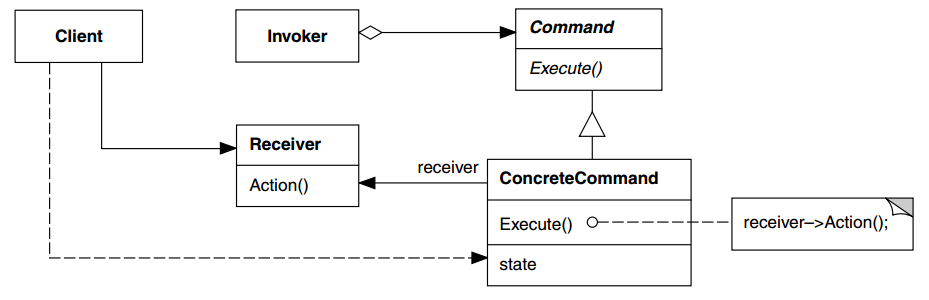
\includegraphics[scale=0.4]{5_padroes-contexto-funcional/5.3_comportamentais/5.3.02_command/diagram.png}
	\end{center}
\end{figure}

\subsection*{Exemplo Orientado a Objetos}

\begin{lstlisting}[caption={Command Orientação a Objetos},label=oocommand]


    
\end{lstlisting}

\subsection*{Contexto Funcional}

\begin{comment}
Por possuir uma definição abrangente com características 
que nem todo domínio utiliza (como enfileiramento de 
commands, operações reversíveis), existe diversas formas 
de implementar o Command. A mais simples, onde é necessário 
apenas implementar uma operação que pode ser chamada em 
um momento futuro do código, é possível através do uso 
de funções de alta ordem. Uma função é definida para 
receber como parâmetro o valor alvo da operação e uma 
função que receba como parâmetro o valor e retorne um 
novo valor do mesmo tipo modificado:

\begin{lstlisting}[caption={Command Funcional},label=fpcommand]
    

    
\end{lstlisting}

Caso seja necessário armazenar diversos Commands em uma 
lista para que eles sejam executados depois, basta que 
a função receba como parâmetro apenas a função que 
realizará a operação, retornando uma nova função que 
deve receber como parâmetro o valor alvo da operação. 
Dessa forma, todos os commands gerados são armazenados em 
uma coleção, por exemplo, uma lista, e os commands 
são aplicados sequencialmente em um valor de entrada, 
onde o valor de saída de uma função é a entrada para a 
próxima, como um pipeline:

\begin{lstlisting}[caption={Coleção de Commands Funcional},label=fpcommands]
    

    
\end{lstlisting}

Implementar a operação de reversão pode ser uma tarefa 
mais complicada. [finalizar para incluir a operação de 
reversão]
\end{comment}
\begin{lstlisting}[caption={Command Reversível},label=fprecommand]
    

    
\end{lstlisting}